\documentclass[main.tex]{subfiles}
\begin{document}

\subsection{Simply typed $\lambda$-calculus with subtyping}
\label{sec:lambda}

In order to be able to represent the notion of generic and specific concepts,
it is well-suited to use some sort of ordering relation over our types.

One such ordering relation is the \emph{subtype} relation, as presented in
\cite[chap.~15]{pierce}, and will be used here.

\begin{example}
    The subtyping construction is particularly useful for domains like
    geographical queries --- it lets us express relations such as the following:
    \begin{align*}
        Capital & \less City \less GSet \\
        Name & \less String \\
        Distance & \less Number \\
    \end{align*}
\end{example}

\subsubsection{Type lattices}
\begin{defn}
    Meet and join:

    We say that $z$ is a \emph{meet} of $x$ and $y$, if:
    \begin{equation}
        z \less x, z \less y,
            \forall t \in X (t \less x, t \less y \implies t \less z)
    \end{equation}

    We say that $z$ is a \emph{join} of $x$ and $y$, if:
    \begin{equation}
        x \less z, y \less z,
            \forall t \in X (x \less t, y \less t \implies z \less t)
    \end{equation}
\end{defn}

\begin{defn}
    A \emph{partial lattice} is a pair $\lattice{ X}{ \less }$ where:
    \begin{itemize}
        \item $\less$ is a partial-order relation
        \item for any $x, y \in X$, there is at most one meet and at most one join.
            They will be denoted as $x \meet y$ (the meet of $x$ and $y$) and
            $x \join y$ (the join of $x$ and $y$).
    \end{itemize}
\end{defn}

\begin{defn}
    A partial lattice $\lattice{ T}{ \less }$ where
    $T \subseteq \tsymbs$ is called a \emph{type lattice}.

    Whenever the relation is unambiguous, $T$ and $\lattice{ T}{ \less }$
    will be used interchangeably: we could say ``let $T$ be a
    type lattice'', which would refer to $\lattice{ T}{ \less }$.
\end{defn}

\begin{defn}
    \label{def:subtype}
    For a type lattice $T$, we extend\footnote{
        To make this completely rigorous, $\mathcal{T}$ would have to be defined
        over \emph{lattices}, not their carrier sets, so that the notion of
        ``extending the relation'' makes sense (because we actually create a
        new relation). These details, however, have been omitted for clarity.
    } the relation
    $\less$ over its type closure:
    \begin{itemize}
        \item $(\sigma \tot \sigma') \less (\tau \tot \tau') \iff (\sigma' \less \sigma)
            \& (\tau \less \tau')$
    \end{itemize}
\end{defn}

\greenbox{
    Note that this definition assumes \emph{contravariant arguments}.
    In essence, the semantics of $f \less g$ is ``wherever we can use $g$,
    we can also use $f$''. Now, imagine that $f : \alpha' \tot \beta'$,
    $g : \alpha'' \tot \beta''$, and we have a function
    $h : (\alpha'' \tot \beta'') \tot \gamma $ that takes $g$ as
    argument and produces something of type $\gamma$. Supposedly,
    $h$ uses $g$ somewhere in its body and supplies it with something
    of type $\alpha''$.

    Now, we supply $f$ to $h$ instead of $g$ --- this $f$ needs to be able
    to take anything of type $\alpha''$ and its subtypes as argument.

    The only way to make this work is to make arguments contravariant,
    while making return values covariant.

    Nevertheless, there exist systems (for example the Dart programming
    language \cite{darttypes}) where covariant arguments are allowed and the
    inconsistencies that
    arise from this decision are left to the user to look out for.
}

\begin{lemma}
    \label{lemma:complexmeet}
    If $T$ is a type lattice and $\sigma = \sigma' \tot \sigma'' \in \tclos{T},
    \tau = \tau' \tot \tau'' \in \tclos{T}$,
    then:
    \begin{enumerate}
        \item \label{loc:fdir} $\eta'$ is a join of $\sigma'$ and $\tau'$ and
            $\eta''$ is a meet of $\sigma''$ and $\tau''$ if and only if
            $\eta' \tot \eta'' = \eta$ is a meet of $\sigma$ and $\tau$.
        \item $\eta'$ is a meet of $\sigma'$ and $\tau'$ and
            $\eta''$ is a join of $\sigma''$ and $\tau''$ if and only if
            $\eta' \tot \eta'' = \eta$ is a join of $\sigma$ and $\tau$.
    \end{enumerate}
\end{lemma}
\begin{proof}
    \begin{comment}
        % actually, this direction is redundant since the other direction
        % proves equivalence
        First, let $\eta'$ be a join of $\sigma'$ and $\tau'$ and
        $\eta''$ be a meet of $\sigma''$ and $\tau''$, e.g:

        \[
            \sigma' \less \eta', \tau' \less \eta',
                \forall \nu \in \tclos{T} (\sigma' \less \nu, \tau' \less \nu \implies \eta' \less \nu)
        \]
        \[
            \eta'' \less \sigma'', \eta'' \less \tau'',
                \forall \nu \in \tclos{T} (\nu \less \sigma'', \nu \less \tau'' \implies \nu \less \eta'')
        \]

        \begin{itemize}
            \item
                since $\sigma' \less \eta'$ and $\eta'' \less \sigma''$, we
                have that $\eta = (\eta' \tot \eta'') \less (\sigma' \tot \sigma'') = \sigma$.
            \item since $\tau' \less \eta'$ and $\eta'' \less \tau''$, we
                have that $\eta = (\eta' \tot \eta'') \less (\tau' \tot \tau'') = \tau$.
            \item let $\nu \in \tclos{T}$ be such that $\sigma \less \nu$
                and $\tau \less \nu$. This means that $\nu = \nu' \tot \nu''$
                such that $\nu' \less \sigma', \nu' \less \tau'$ and
                $\sigma'' \less \nu'', \tau'' \less \nu''$.

                But since $\eta'$ is a join of $\sigma'$ and $\tau'$, we know
                that $\eta' \less \nu'$. And dually,
                since $\eta''$ is a meet of $\sigma''$ and $\tau''$, we know
                that $\nu'' \less \eta''$.

                Then, we have that $\nu \less \eta$.
        \end{itemize}
    \end{comment}

    We will prove both directions of (\ref{loc:fdir}) by applying equivalent
    transformations:

    $\eta$ being a meet of $\sigma$ and $\tau$ is defined as:
    \[
        \eta \less \sigma, \eta \less \tau,
            \forall \nu \in \tclos{T} (\nu \less \sigma, \nu \less \tau \implies \nu \less \eta)
    \]
    Now, expand the complex types:
    \[    (\eta' \tot \eta'') \less (\sigma' \tot \sigma''),
    \]
    \[    (\eta' \tot \eta'') \less (\tau' \tot \tau''),
    \]
    \[
            \forall (\nu' \tot \nu'') \in \tclos{T} ((\nu' \tot \nu'') \less (\sigma' \tot \sigma''), (\nu' \tot \nu'') \less (\tau' \tot \tau'') \implies (\nu' \tot \nu'') \less (\eta' \tot \eta''))
    \]
    Then apply \cref{def:subtype}:
    \[    (\sigma' \less \eta') , (\eta'' \less \sigma'')
    \]
    \[    (\tau' \less \eta') , (\eta'' \less \tau'')
    \]
    \[
            \forall (\nu' \tot \nu'') \in \tclos{T}
            ((\sigma' \less \nu'), (\nu'' \less \sigma''),
             (\tau' \less \nu'), (\nu'' \less \tau'')
             \implies (\eta' \less \nu'), (\nu'' \less \eta''))
    \]
    Now, split the third condition (properties of universal quantification and implication)
    and rearrange the lines:
    \[
        \sigma' \less \eta', \tau' \less \eta',
            \forall \nu \in \tclos{T} (\sigma' \less \nu, \tau' \less \nu \implies \eta' \less \nu)
    \]
    \[
        \eta'' \less \sigma'', \eta'' \less \tau'',
            \forall \nu \in \tclos{T} (\nu \less \sigma'', \nu \less \tau'' \implies \nu \less \eta'')
    \]
    This is exactly the condition that $\eta'$ is a join of $\sigma'$
    and $\tau'$ and
    $\eta''$ is a meet of $\sigma''$ and $\tau''$.

    The argument for joins is dual to the one for meets and is, therefore, omitted for brevity.
\end{proof}

\begin{prop}
    \label{prop:typelattice}
    If $T$ is a type lattice, then $\tclos{T}$ is a partial lattice.
\end{prop}
\begin{proof}
    Let $\sigma, \tau \in \tclos{T}$. We will inductively (by their syntactic
    structure) prove that they have at most one join or meet.

    First, let $\eta_1$ and $\eta_2$ be meets of $\sigma$ and $\tau$.
    Since $\less$ is only defined if operands have the same syntactic structure
    and we have that $\eta_1 \less \sigma, \eta_1 \less \tau, \eta_2 \less \sigma, \eta_2 \less \tau$,
    they are all forced to have the same syntactic structure. Thus, there are
    two possibilities:

    \begin{itemize}
        \item $\sigma, \tau, \eta_1, \eta_2 \in T$:

            since $T$ is a partial
            lattice, $\sigma$ and $\tau$ have a unique meet. Thus, $\eta_1 = \eta_2$.
        \item $\sigma = \sigma' \tot \sigma'', \tau = \tau' \tot \tau'',
            \eta_1 = \eta'_1 \tot \eta'_1, \eta_2 = \eta'_2 \tot \eta'_2$:

            Since $\eta_1$ and $\eta_2$ are meets of $\sigma$ and $\tau$, we have
            by \cref{lemma:complexmeet} that $\eta'_1$ and $\eta'_2$ are meets
            of $\sigma'$ and $\tau'$, and that $\eta''_1$ and $\eta''_2$ are meets
            of $\sigma''$ and $\tau''$.

            Inductively, $\eta'_1 = \eta'_2$ and $\eta''_1 = \eta''_2$. Thus,
            $\eta_1 = \eta'_1 \tot \eta''_1 = \eta'_2 \tot \eta''_2 = \eta_2$.
    \end{itemize}

    The argument for joins is dual to the argument for meets and is again
    omitted.
\end{proof}

\begin{property}
    For a type lattice $T$, and arbitrary $\sigma = \sigma' \tot \sigma'' \in \tclos{T}
    , \tau = \tau' \tot \tau'' \in \tclos{T}$, we have:
    \[
        \sigma \meet \tau \condeq (\sigma' \join \sigma'') \tot (\tau' \meet \tau'')
    \]
    \[
        \sigma \join \tau \condeq (\sigma' \meet \sigma'') \tot (\tau' \join \tau'')
    \]
    (where $\condeq$ means ``either both sides are defined and equal or both are
    undefined'')
\end{property}
\begin{proof}
    This follows directly from \cref{lemma:complexmeet} and the proof of
    \cref{prop:typelattice}.
\end{proof}


\subsubsection{Terms}
We will now extend the definition of $\lambda$-term given in \cref{purelambda:types}
to work with subtypes.

We need this in order to extend type systems with additional information,
and to be able to dispose of the extra information when it is no longer needed.

So, for a of type lattice $T$, we will define the set of
\emph{pre-typed $\lambda$-terms with subtypes} ($\fancylambda{T}{C}$).

\begin{defn}
    Let $C \subset \const$ be a set of constants, typed in $T$.

    $\fancylambda{T}{C}$ is defined inductively:
    \begin{itemize}
        \item Constant:    \[ c \in C \implies c \in \fancylambda{T}{C} \]
        \item Variable:    \[ v \in \lvars \implies v \in \fancylambda{T}{C} \]
        \item Application: \[ A, B \in \fancylambda{T}{C} \implies (AB) \in \fancylambda{T}{C} \]
        \item Abstraction: \[ v \in \lvars, A \in \fancylambda{T}{C}, \sigma \in \tclos{T}
                \implies (\lambda v : \sigma \abstr A) \in \fancylambda{T}{C} \]
        \item Construction: \[ \sigma \in T, A \in \fancylambda{T}{C}
                \implies \sigma[A] \in \fancylambda{T}{C} \]
    \end{itemize}
\end{defn}

\begin{defn}
    \label{def:subtypederiv}
    Derivation rules for $\lambda$-calculus with subtypes:

    \begin{itemize}
        \item Constant
            \cenderiv{
                \hypo{c \in C}
                \infer1{\Gamma \vdash c : \typeof{c}}
            }
        \item Variable
            \cenderiv{
                \hypo{x : \sigma \in \Gamma}
                \infer1{\Gamma \vdash x : \sigma}
            }
        \item Application
            \cenderiv{
                \hypo{\Gamma \vdash A : \sigma' \tot \sigma''}
                \hypo{\Gamma \vdash B : \tau}
                \hypo{\tau \less \sigma'}
                \infer3{\Gamma \vdash (AB) : \sigma''}
            }
        \item Abstraction
            \cenderiv{
                \hypo{\Gamma \circ x : \tau \vdash A : \sigma}
                \infer1{\Gamma \vdash (\lambda x : \tau \abstr A) : \tau \tot \sigma}
            }
        \item Construction via upcast
            \cenderiv{
                \hypo{\Gamma \vdash A : \sigma}
                \hypo{\sigma \less \tau}
                \infer2{\Gamma \vdash \tau[A] : \tau}
            }
        \item Construction via downcast (dangerous, doesn't need to be included in most cases\fixednote{не видях в текста никъде да използваш downcast, ако наистина е така, може би е по-добре да го махнеш}            \cenderiv{
                \hypo{\Gamma \vdash A : \sigma}
                \hypo{\tau \less \sigma}
                \infer2{\Gamma \vdash \tau[A] : \tau}
            }
    \end{itemize}
\end{defn}

Now we will show that every well-typed term has a unique type under a fixed context:
\begin{prop}
    \label{prop:uniquetypes}
    \[ \Gamma \vdash M : \sigma' \land \Gamma \vdash M : \sigma''
        \implies \sigma' = \sigma'' \]
\end{prop}
\begin{proof}
    Assume $\Gamma \vdash M : \sigma'$ and $\Gamma \vdash M : \sigma''$
    and prove this by induction over the construction of $M$:
    \begin{itemize}
        \item The proof for Constant, Variable, Application, and Abstraction is identical
            to the one for \cref{prop:uniquetypes}

        \item $M = \sigma[A]$: this directly means that $\sigma' = \sigma = \sigma''$.
    \end{itemize}
\end{proof}

\subsubsection{Type set subsumption}
We will now formalise the notion of a type lattice being more general
or more concrete than another type lattice.

\begin{defn}
    If $\lattice{ T}{ \less' }$ and $\lattice{ S}{ \less }$
    are type lattices, we say that $\lattice{ T}{ \less' } \tless \lattice{ S}{ \less }$ if:
    \begin{itemize}
        \item $S \subseteq T$
        \item $\less \subseteq \less'$ and $\restr{\less'}{S \times S} = \less$
        \item $\forall \tau \in (T \setminus S) ((\exists \sigma \in S : \tau \less \sigma )
            \xor (\exists \sigma \in S : \sigma \less \tau)$
    \end{itemize}
    (where $\xor$ means logical ``exclusive or'')
\end{defn}

Essentially, this says that $T$ subsumes, or encompasses, $S$: any type in
$T$ is either a more concrete variant or a more general variant of some type in $S$.

If $\tau\in T$ is such that $(\exists \sigma \in S : \tau \less \sigma)$, we will
call $\tau$ \emph{special}. Dually, if $\tau\in T$ is such that
$(\exists \sigma \in S : \sigma \less \tau)$, we will call $\tau$
\emph{general}.

If we have $T \tless S$, it would be convenient to be able to convert between them.
The conversion from $S$ to $T$ is trivial. The conversion from $T$ to $S$,
however, involves discarding information.

\begin{example}
    For example, let $S = \{ Int, String \}$, supposing the obvious semantics
    behind those names. This is a nice type system --- however, one might want to
    be able to encode extra information within types: this comes especially
    handy in the context of CCGs.

    So, we add some extra types: \[ T = \{ Int, String, Distance, Count, NamedEntity \} \]
    We want $\less$ to be defined as \[ Distance \less Int, Count \less Int,
    NamedEntity \less String \]

    Now while doing natural language parsing, we can use $T$. Afterwards
    we no longer need the extra information, so we could discard the extra
    types and return to $S$. To do this, we define a \emph{squash function}.
\end{example}

\begin{defn}\label{def:squashfn}
    $\squash: T \fun S$ is a \emph{squash function} for
    $\lattice{ T}{ \less' } \tless \lattice{ S}{ \less }$, if:
    \begin{itemize}
        \item for each $\tau \in S$, $\squash(\tau) = \tau$
        \item it follows the subtyping relation:
            \[ \forall \sigma \in T
                (\squash(\sigma) \less' \sigma \lor \sigma \less' \squash(\sigma)) \]
        \item it preserves the subtyping relation:
            \[ \forall \sigma, \tau \in T (\sigma \less' \tau \implies
                \squash(\sigma) \less \squash(\tau)) \]
    \end{itemize}
\end{defn}

\begin{property}
    \label{prop:squash:preserve}
    Squash functions preserve the subtyping relation for complex types:
    \[ \forall \sigma, \tau \in \tclos{T} (\sigma \less' \tau \implies
        \tsquash(\sigma) \less \tsquash(\tau)) \]
\end{property}
\begin{proof}
    First, assume $\sigma \less' \tau$.

    The property is proven by induction over the construction of $\sigma$
    and $\tau$.

    \begin{itemize}
        \item $\sigma \in T, \tau \in T$: this is true by definition.
        \item $\sigma = (\sigma' \tot \sigma''), \tau = (\tau' \tot \tau'')$:
            since $\sigma \less' \tau$, we have that $\tau' \less' \sigma'$
            and $\sigma'' \less' \tau''$.

            Therefore, inductively, $\tsquash(\tau') \less \tsquash(\sigma')$
            and $\tsquash(\sigma'') \less \tsquash(\tau'')$. Thus,
            \[
                \tsquash(\sigma) = (\tsquash(\sigma') \tot \tsquash(\sigma''))
                \less
                (\tsquash(\tau') \tot \tsquash(\tau'')) = \tsquash(\tau)
            \]
        \item in other cases, $\sigma$ and $\tau$ have different syntactic
            structure and $\less'$ is not defined. Since $\tsquash$ preserves
            syntactic structure, $\tsquash(\sigma)$ and $\tsquash(\tau)$
            will also have different syntactic structure, thus $\less$ will
            be undefined for them as well.
    \end{itemize}
\end{proof}

\begin{property}\label{prop:squashminmax}
    If $\squash: T \fun S$ is a squash function for
    $\lattice{ T}{ \less' } \tless \lattice{ S}{ \less }$,
    then $\squash(\tau) = min_{\less} \{ \sigma \in S \mid \tau \less' \sigma \}$
    for special elements $\tau \in T \setminus S$, and dually
    $\squash(\tau) = max_{\less} \{ \sigma \in S \mid \sigma \less' \tau \}$.
    for general elements $\tau \in T \setminus S$.
\end{property}
\begin{proof}
    WLOG\footnote{The argument for general elements is dual to the one for special
        elements.},
    let $\tau$ be a special element in $T \setminus S$, e.g. for every
    $\sigma \in S$ that $\tau$ is comparable with, $\tau \less' \sigma$.

    Now, since $\squash(\tau)$ is comparable with $\tau$, we have
    $\tau \less' \squash(\tau)$.

    Let $\sigma \in S$ be an arbitrary element such that $\tau \less' \sigma$.
    By the preservation property of $\squash$, we know that
    $\tau \less' \squash(\tau) \less \squash(\sigma) = \sigma$.

    Thus, $\squash(\tau)$ is lower-than any element that is comparable
    by $\less$ with any element that is comparable by $\less'$ with $\tau$.
    This gives that $\squash(\tau)$ is the minimal element in $S$ that is
    greater-than $\tau$.
\end{proof}
\begin{corollary}\label{prop:squash:unique}
    If there is a squash function $\squash: T \fun S$ for
    $\lattice{ T}{ \less' } \tless \lattice{ S}{ \less }$,
    it is unique in the sense that there is no other squash function for
    $\lattice{ T}{ \less' } \tless \lattice{ S}{ \less }$.
\end{corollary}
\begin{proof}
    The value of $\squash(\tau)$ is unambiguous in all cases:
    \begin{itemize}
        \item If $\tau \in S$, then $\squash(\tau) = \tau$
        \item If $\tau \in T \setminus S$ and $\tau$ is special
            then $\squash(\tau) = min_{\less} \{ \sigma \in S \mid \tau \less' \sigma \}$
        \item If $\tau \in T \setminus S$ and $\tau$ is general
            then $\squash(\tau) = max_{\less} \{ \sigma \in S \mid \sigma \less' \tau \}$
    \end{itemize}
\end{proof}

\begin{property}\label{prop:squashcomp}
    The composition of two squash functions is a squash function, i.e. if:
    \begin{itemize}
        \item $\squash' : T' \fun T$ is a squash function for
            $\lattice{T'}{\less'} \tless \lattice{T}{\less}$
        \item $\squash'' : T'' \fun T'$ is a squash function for
            $\lattice{T''}{\less''} \tless \lattice{T'}{\less'}$
    \end{itemize}
    Then $\squash \defeq \squash' \circ \squash''$ is a squash function
    for $\lattice{T''}{\less''} \tless \lattice{T}{\less}$.
\end{property}
\begin{proof}
    We will prove the squash function properties of $\squash$ one by one:
    \begin{itemize}
        \item for each $\tau \in T$, $\squash(\tau) = \tau$:

            We have that $\squash(\tau) = \squash'(\squash''(\tau))$.
            Since $T'' \tless T' \tless T$ implies $T'' \supseteq T' \supseteq T$,
            then $\tau \in T$ implies $\tau \in T'$. Also, $\squash''(\tau) = \tau$.
            Thus, $\squash'(\squash''(\tau)) = \tau$.

        \item it follows the subtyping relation:
            \[ \forall \sigma \in T''
                (\squash(\sigma) \less'' \sigma \lor \sigma \less'' \squash(\sigma)) \]

            From the same property for $\squash'$ and $\squash''$, we have 2 cases:
            \begin{itemize}
                \item Both relations are in the same direction,
                    WLOG $\squash''(\tau) \less'' \tau$ and
                    $\squash'(\squash''(\tau)) \less' \squash''(\tau)$:


                    This means that $\squash'(\squash''(\tau)) \less'' \tau$.

                \item The two relations are in different directions,
                    WLOG $\tau \less'' \squash''(\tau)$ and
                    $\squash'(\squash''(\tau)) \less' \squash''(\tau)$:

                    In this case, $\squash''(\tau)$ is both general for $T' \tless T$ 
                    (because it is greatest in $T'$ because of \cref{prop:squashminmax})
                    and special for $T' \tless T$ (because it is lesser than
                    $\squash'(\squash''(\tau)) \in T$).

                    This means that $\tau \in T$, which makes the property trivial.
            \end{itemize}

        \item it preserves the subtyping relation:
            \[ \forall \sigma, \tau \in T'' (\sigma \less'' \tau \implies
                \squash(\sigma) \less \squash(\tau)) \]

            Let $\sigma, \tau \in T''$ be fixed such that $\sigma \less'' \tau$.
            We have that $\squash''(\sigma) \less' \squash''(\tau)$ because
            $\squash''$ preserves $\less''$. Subsequently, since $\squash'$
            preserves $\less'$, we have that $\squash'(\squash''(\sigma))
            \less \squash'(\squash''(\tau))$.
    \end{itemize}
\end{proof}

We can now naturally extend squash functions to work over $\lambda$-terms
and contexts:
\begin{defn}
    If $\squash: T \fun S$ is a squash function for $T \tless S$ and
    $C$ is typed in $S$,
    $\lsquash: \fancylambda{T}{C} \fun \fancylambda{S}{C}$
    is defined inductively:

    \[
        \lsquash(A) =
        \begin{cases*}
            c ,& $A = c \in C$ \\
            v ,& $A = v \in \lvars$ \\
            \lsquash(M) \lsquash(N) ,& $A = (MN)$ \\
            \lambda x : \tsquash(\sigma) \abstr \lsquash(M)
 ,& $A = \lambda x : \sigma \abstr M$ \\
                \tsquash(\sigma)[M] ,& $A = \sigma[M]$ \\
        \end{cases*}
    \]

    Also,
    $\consquash$, which operates on contexts
    is defined as follows:

    \[
        \consquash(\Gamma)
            = \{ x : \tsquash(\sigma) \mid (x : \sigma) \in \Gamma \}
    \]
\end{defn}

From here on $\squash$ may be used freely in place of $\lsquash$
and $\consquash$.

And now, the main proposition of this section, which tells us that when
dropping a well-typed $\lambda$-term from an extended type system into
a basic type system, it remains well-typed and has a useful type.
In the implementation this is used for dropping from the user-defined
type system used for CCG parsing into the Minipass type system
(\cref{sec:termgen}).

\begin{prop}
    For a squash function $\squash: T \fun S$, $\lsquash$ is
    well-defined, namely
    \[ \Gamma \vdash A : \sigma \implies
        \consquash(\Gamma) \vdash \lsquash(A) : \tsquash(\sigma) \]
\end{prop}
\begin{proof}
    Let $\Gamma \vdash A : \sigma$. We will now prove the right-hand side
    by induction over the construction of $A$:
    \begin{itemize}
        \item $A = c \in C$. This means that $\typeof{c} = \sigma$ and thus
            $\sigma \in \tclos{S}$ because $C$ is typed in S: therefore
            $\tsquash(\sigma) = \sigma$. Also, we have that $\lsquash(c) = c$,
            and so \[ \Gamma \vdash c : \sigma \implies
                \consquash(\Gamma) \vdash c : \sigma \implies
                \consquash(\Gamma) \vdash \lsquash(c) : \tsquash(\sigma) \]

        \item $A = v \in \lvars$. We have that $(v : \sigma) \in \Gamma$, thus
            $(v : \tsquash(\sigma)) \in \consquash(\Gamma)$. But $\lsquash(v) = v$,
            so $\consquash(\Gamma) \vdash \lsquash(v) : \tsquash(\sigma)$.

        \item $A = (MN)$, where $\Gamma \vdash M : (\eta' \tot \sigma)$
            and $\Gamma \vdash N : \eta$ where $\eta \less \eta'$.

            Inductively, we know that
            \begin{equation}
                \consquash(\Gamma) \vdash \lsquash(M) : (\tsquash(\eta')
                    \tot \tsquash(\sigma))
            \end{equation}
            \begin{equation}
                \consquash(\Gamma) \vdash \lsquash(N) : \tsquash(\eta)
            \end{equation}

            And by \cref{prop:squash:preserve} we have that $\tsquash(\eta)
                \less \tsquash(\eta')$.

            Finally, by the application rule of \cref{def:subtypederiv},
            we have that $\consquash(\Gamma) \vdash (\lsquash(M) \lsquash(N))
            : \tsquash(\sigma) $

        \item $A = (\lambda x : \tau \abstr M)$, where $\Gamma' = \Gamma \circ
            (x : \tau) \vdash M : \eta$ and $\sigma = \tau \tot \eta$.

            Inductively, we have that $\consquash(\Gamma') \vdash \lsquash(M) : \tsquash(\eta)$.
            However, $\consquash(\Gamma') = \consquash(\Gamma) \circ (x : \tsquash(\tau))$,
            therefore \[ \consquash(\Gamma) \vdash (\lambda x : \tsquash(\eta)
                \abstr \lsquash(M)) : \tsquash(\tau) \tot \tsquash(\eta) = \tsquash(\sigma) \]

        \item $A = \sigma[M]$, where $\Gamma \vdash M : \tau$.

            Inductively, we have $\consquash(\Gamma) \vdash \lsquash(M) : \tsquash(\tau)$.

            Since either $\sigma \less \tau$ (upcast) or $\tau \less \sigma$
            (downcast), by \cref{prop:squash:preserve} we have that either
            $\tsquash(\sigma) \less \tsquash(\tau)$ or $\tsquash(\tau) \less \tsquash(\sigma)$.

            Thus, \[
                \consquash(\Gamma) \vdash \tsquash(\sigma)[\lsquash(M)] : \tsquash(\sigma)
            \]
    \end{itemize}
\end{proof}

\subsubsection{Subtype libraries}
\begin{defn}
    A statement in the form $\sigma \lass \tau (\sigma, \tau \in \tsymbs)$
    is called a \emph{subtype assertion}.
\end{defn}

Since our definition of ``subtype'' doesn't allow us to subtype a complex type,
we have to work around this by making $\sigma$ be a complex type with the same
syntactic structure as $\tau$ and then subtyping on the level of individual
basic types it is made of. To do this, we need to be able to create a new term
with the same syntactic structure of another term.

\begin{example}
    Suppose we have the basic types $Int$ and $String$, and we want to extend
    them.

    For example, take the subtype assertion $F \lass ( Int \tot String )$.
    Let $\tau = ( Int \tot String )$. We want $F$ to correspond to a type
    $\sigma$ such that $\sigma \less \tau$. To do this, we clone
    the complex type $\tau$, creating a new type with the same
    syntactic structure: $\sigma = ( Int' \tot String' )$

    Now we extend our subtyping relation to include $ Int \less Int', String' \less String $,
    which indeed gives that $\sigma \less \tau$.

    Again, take note of the argument contravariance.

    To remember that $F$ stands for $\sigma$, we will iteratively build a
    function $\varphi$ such that $\varphi(F) = \sigma$.
\end{example}

The following few definitions will formalise this process.

First, having a type $\tau$, we need to be able to create a new type
that is its clone
(has the same syntactic structure), and is a subtype of $\tau$.

To deal with contravariance, we will differentiate between a ``subtype clone''
($\subtyper{clone}$)
that clones a type into a new one that will be its subtype, and a
``supertype clone'', ($\suptyper{clone}$)
that dually creates a ``supertype'' clone --- in this way we will be able to
use the $\suptyper{clone}$ in arguments and $\subtyper{clone}$ in return
values.

To do this, we will use the mappings $\subtyper{\xi}$ and $\suptyper{\xi}$
that rename the basic types used in $\tau$ into new type symbols. To clone
$\tau$, we will recursively replace argument types and return value types
with their respective clones. One way to deal with contravariance is the following:

\newcommand\clonesub{\subtyper{clone}_{\subtyper{\xi} \suptyper{\xi}}}
\newcommand\clonesup{\suptyper{clone}_{\subtyper{\xi} \suptyper{\xi}}}

\begin{defn}
    Let $\lattice{ T}{ \less }$ be a type lattice, $\tau \in \tclos{T}$
    be a type and $\subtyper{\xi}, \suptyper{\xi}$ be mappings from a
    superset of
    $\ts{\tau}$ into $\tsymbs$ such that
    $range(\suptyper{\xi}) \cap range(\subtyper{\xi}) = \emptyset$.

    $\suptyper{clone}_{\subtyper{\xi} \suptyper{\xi}}$ and
    $\subtyper{clone}_{\subtyper{\xi} \suptyper{\xi}}$ are defined by
    mutual recursion:

    \[
        \subtyper{clone}_{\subtyper{\xi} \suptyper{\xi}}(\tau) =
        \begin{cases*}
            \subtyper{\xi}(\tau) ,&
                $\tau \in T$ \\
            \suptyper{clone}_{\subtyper{\xi} \suptyper{\xi}}(\tau_1)
                \tot \subtyper{clone}_{\subtyper{\xi} \suptyper{\xi}}(\tau_2) ,&
                $\tau = \tau_1 \tot \tau_2$ \\
        \end{cases*}
    \]

    \[
        \suptyper{clone}_{\subtyper{\xi} \suptyper{\xi}}(\tau) =
        \begin{cases*}
            \suptyper{\xi}(\tau) ,&
                $\tau \in T$ \\
            \subtyper{clone}_{\subtyper{\xi} \suptyper{\xi}}(\tau_1)
                \tot \suptyper{clone}_{\subtyper{\xi} \suptyper{\xi}}(\tau_2) ,&
                $\tau = \tau_1 \tot \tau_2$ \\
        \end{cases*}
    \]

\end{defn}

\begin{property}
    \label{prop:clone:rel}
    If we have $\forall \eta (\subtyper{\xi}(\eta) \less \eta)$ and
    $\forall \eta (\eta \less \suptyper{\xi}(\eta))$, then for
    any $\tau$:
    \begin{itemize}
        \item $\clonesub(\tau) \less \tau$
        \item $\tau \less \clonesup(\tau)$
    \end{itemize}
\end{property}
\begin{proof}
    This property is proven by induction over the structure of $\tau$:

    \begin{itemize}
        \item $\tau \in T$:
            \begin{itemize}
                \item $\clonesub(\tau) = \subtyper{\xi}(\tau) \less \tau$
                \item $\tau \less \suptyper{\xi}(\tau) = \clonesup(\tau)$
            \end{itemize}
        \item $\tau = \tau_1 \tot \tau_2$:
            \begin{itemize}
                \item Since inductively $\tau_1 \less \clonesup(\tau_1)$
                    and $\clonesub(\tau_2) \less \tau_2$, by \cref{def:subtype}
                    we have that:
                    \[ \clonesub(\tau) = \clonesup(\tau_1) \tot \clonesub(\tau_2)
                    \less \tau_1 \tot \tau_2 = \tau. \]
                \item Since inductively $\clonesub(\tau_1) \less \tau_1$
                    and $\tau_2 \less \clonesup(\tau_2)$, by \cref{def:subtype}
                    we have that:
                    \[ \tau = \tau_1 \tot \tau_2 \less
                    \clonesub(\tau_1) \tot \clonesup(\tau_2) = \clonesup(\tau). \]
            \end{itemize}
    \end{itemize}
\end{proof}

Now we will define an iterative process for adding new types into a type lattice
by subtyping existing types.

Suppose we have the subtype assertion $\sigma \lass \tau$ with the intent of adding
a new type ``$\sigma$'' to $T$ such that $\sigma \less \tau$. We are unable to add $\sigma$
to $T$ directly, since this would require subtyping a type with a different syntactic
structure. So, instead we will construct another type $\varphi(\sigma) \in \tclos{T}$
whose constituent atomic types we add to $T$.

We will now define the operation $\tadd$ that does exactly that.

Afterwards, when we need to refer to $\tau$, we will use $\varphi(\sigma)$.

Since we want to be able to define several new types one after the other,
$\tadd$ will need to use the existing mapping $\varphi$ to interpret
existing manually-constructed types, and extend it with the new type.
\begin{defn}
    \label{def:subadd}
    Given
    \begin{itemize}
        \item a type lattice $\lattice{ T}{ \less }$
        \item a type symbol $\sigma \in \tsymbs \setminus T$
        \item a mapping $\varphi : T \fun \tclos{T}$\fixednote{тук означението $\pfun$ се появява за пръв път без да е обяснено, не мисля че може да се счита стандартно означение на частична функция.}
        \item a type $\tau$ such that $\hat{\varphi}(\tau)$ is defined\fixednote{ако започваш от $\varphi = \emptyset$ това условие няма как да е изпълнено}
    \end{itemize}
    Let $\suptyper{\xi}$ and $\subtyper{\xi}$ be injections from
    $\ts{\hat{\varphi}(\tau)}$ into $\tsymbs \setminus (T \cup \{ \sigma \})$ such that
    $range(\suptyper{\xi}) \cap range(\subtyper{\xi}) = \emptyset$\footnote{
        $\suptyper{\xi}$ and $\subtyper{\xi}$ depend on $\tau$, $T$ and
        $\sigma$. If one wants to make their choice constrictive, they may,
        for example, assume that $\tsymbs$ is ordered, take the minimal
        elements that aren't in $T \cup \{ \sigma \}$ and map to them in
        order.
    }.

    Now define the operation $\tadd$ as:
        \[ \langle \lattice{ T}{ \less }, \varphi \rangle
            \tadd (\sigma \lass \tau)
            \defeq
            \langle \lattice{ T'}{ \less' }, \varphi' \rangle
        \] where:
    \begin{itemize}
        \item $\rho = \clonesub(\hat{\varphi}(\tau))$
        \item $T' = T \cup ((range(\subtyper{\xi}) \cup range(\suptyper{\xi})) \cap \ts{\rho})$
        \item $\less'$ is the transitive and reflexive closure of
            $\less \cup \{ (\sigma', \tau') \in T' \times T \mid \subtyper{\xi}(\tau') = \sigma' \}
                   \cup \{ (\sigma', \tau') \in T \times T' \mid \suptyper{\xi}(\sigma') = \tau' \}$
        \item $\varphi' = \varphi \cup \{ (\sigma, \rho) \}$
    \end{itemize}

    Note: in the cases where $\varphi$ is irrelevant, it will be omitted as
    so:
    \[ \lattice{ T}{ \less }
        \tadd (\sigma \lass \tau)
        \defeq
        \lattice{ T'}{ \less' }
    \]
\end{defn}

\begin{property}
    Objects constructed by $\tadd$ are correct type lattices.
\end{property}
\begin{proof}
    We extend $\less$ only by adding single edges (and their transitive and
    reflective closure) to new vertices, which creates a ``tree-like'' extension.
    There is no way to introduce a double join or meet, since this would
    require adding more than one edge to a new vertex.
\end{proof}

\begin{lemma}
    \label{lemma:subadd:rel}
    If $\lattice{ T}{ \less }$ is a type lattice, $\theta = (\sigma \lass \tau)$
    is a subtype assertion satisfying the conditions from \cref{def:subadd}
    and $\lattice{ T'}{ \less' } = \lattice{ T}{ \less } \tadd \theta$, then
    \[ T' \tless T \]
\end{lemma}
\begin{proof}
    Let $\subtyper{\xi}$ and $\suptyper{\xi}$ be the injections from \cref{def:subadd}.
    Now, we check the conditions for $T' \tless T$:
    \begin{itemize}
        \item $T \subseteq T'$:

            this is true by definition (
            $T' = T \cup ((range(\subtyper{\xi}) \cup range(\suptyper{\xi})) \cap \ts{\rho})$
            ) where $range(\subtyper{\xi})$ and $range(\suptyper{\xi})$ contain
            only fresh symbols (not in $T$).

        \item $\less \subseteq \less'$:

            $\less'$ contains $\less$ by definition.

        \item $\restr{\less'}{S \times S} = \less$:

            we only add edges to $\less$ that point to symbols that are not
            in $T$. Moreover, the transitive and reflexive closures do not
            affect this condition because $\less$ is already transitive and
            reflexive.

        \item $\forall \tau \in (T' \setminus T) ((\exists \sigma \in T : \tau \less' \sigma )
            \xor (\exists \sigma \in T : \sigma \less' \tau)$:

            Fix an arbitrary $\tau \in (T' \setminus T)$.

            Since $T' \setminus T$ is comprised of elements from the ranges
            of $\subtyper{\xi}$ and $\suptyper{\xi}$, there are two options
            for $\tau$:
            \begin{itemize}
                \item $\tau \in range(\subtyper{\xi})$: this means that
                    $\subtyper{\xi}(\sigma) = \tau$ for some $\sigma \in T$, but that
                    also means that we have set $\tau \less' \sigma$.
                \item $\tau \in range(\suptyper{\xi})$: this means that
                    $\suptyper{\xi}(\sigma) = \tau$ for some $\sigma \in T$, but that
                    also means that we have set $\sigma \less' \tau$.
            \end{itemize}

            The exclusive ``or'' is satisfied because
            $range(\subtyper{\xi}) \cap range(\suptyper{\xi}) = \emptyset$.
    \end{itemize}
\end{proof}

\begin{lemma}
    \label{lemma:subadd:phi}
    If $\lattice{ T}{ \less }$ is a type lattice, $\theta = (\sigma \lass \tau)$
    is a subtype assertion and $\varphi$ is a function, both of which satisfy the conditions from \cref{def:subadd}
    and $\langle \lattice{ T'}{ \less' }, \varphi' \rangle
    = \langle \lattice{ T}{ \less }, \varphi \rangle \tadd \theta$, then
    \[ \varphi'(\sigma) \less' \hat{\varphi}(\tau). \]
\end{lemma}
\begin{proof}
    Let $\subtyper{\xi}$ and $\suptyper{\xi}$ be the injections from \cref{def:subadd}.

    We know that $\varphi'(\sigma) = \clonesub(\hat{\varphi}(\tau))$.

    Moreover,
    $\forall \eta (\subtyper{\xi}(\eta) \less' \eta)$ and
    $\forall \eta (\eta \less' \suptyper{\xi}(\eta))$ by the construction of
    $\less'$.

    Then, by \cref{prop:clone:rel} we have that $\varphi'(\sigma) \less'
    \hat{\varphi}(\tau)$.
\end{proof}

\begin{defn}
    A finite sequence of subtype assertions
    $\Theta_T = \theta_1 ... \theta_n$ is called a \emph{subtype library} over $T$
    if the construction $\hat{\Theta}_T \defeq \langle \lattice{ T}{ \less }, \identity_T \rangle \oplus \theta_1 \oplus \theta_2 ... \oplus \theta_n$
    is defined\fixednote{тук не става ясно, че освен понятието ``subtype library'' дефинираш също и $\hat{\Theta}_T$} \footnote{
        When trying to redefine a previously defined type, the sequence is not
        a subtype library because of the restriction for $\sigma$
        in \cref{def:subadd}.
    }.

    Also, we can define the function that gives us all the new type names
    asserted by the subtype library as
    $left(\Theta_T) = \{ \sigma \mid \sigma \lass \tau \in \Theta_T \}$
\end{defn}

\begin{prop}
    If $T$ is a type lattice and
    $\Theta_T = \theta_1 ... \theta_n$ is a subtype library over $T$, where
    $\hat{\Theta}_T = \langle \lattice{ T'}{ \less' }, \varphi \rangle$
    the following properties hold:
    \begin{itemize}
        \item $dom(\varphi) = T \cup left(\Theta)$
        \item $\sigma \less \tau \implies \sigma \less' \tau$
        \item $\sigma \lass \tau \in \Theta \implies \varphi(\sigma) \less' \hat{\varphi}(\tau)$
    \end{itemize}
\end{prop}
\begin{proof}
    We will check all conditions one by one:
    \begin{itemize}
        \item $dom(\varphi) = T \cup left(\Theta)$ (and $\varphi$ is defined correctly):

            Initially, $dom(\varphi) = \identity_T$.
            For every $\sigma \lass \tau \in \Theta$, we have added
            $(\sigma, \rho)$ to $\varphi$ for some $\rho$ in $\tclos{T'}$.

            Thus, we never violate the domain constraint for $\varphi$.

        \item $\sigma \less \tau \implies \sigma \less' \tau$:

            This is true because
            at each step we only add elements to the relation.
        \item $\sigma \lass \tau \in \Theta \implies \varphi(\sigma) \less' \hat{\varphi}(\tau)$:

            Let $\sigma \lass \tau = \theta_i$.

            We have that
            $\langle \lattice{ T'}{ \less' }, \varphi \rangle
                = \langle \lattice{ T}{ \less }, \identity_T \rangle
                \tadd \theta_1 \tadd ... \tadd \theta_i \tadd ... \tadd \theta_n$

            Let
            $\langle \lattice{ T^{(i)}}{ \less^{(i)} }, \varphi^{(i)} \rangle
                = \langle \lattice{ T}{ \less }, \identity_T \rangle
                \tadd \theta_1 \tadd ... \tadd \theta_i$ \quad ($T' = T^{(n)},
                \less' = \less^{(n)}$).

            Since $\Theta$ is a valid subtype library, we know that
            $\hat{\varphi}^{(i - 1)}(\tau) \in \tclos{T^{(i - 1)}}$.

            By \cref{lemma:subadd:phi} $\varphi^{(i)}(\sigma) \less^{(i)}
            \hat{\varphi}^{(i - 1)}(\tau)$. Since $\varphi$ is constructed
            incrementally, we also have $\varphi^{(n)}(\sigma) \less^{(n)}
            \hat{\varphi}^{(n)}(\tau)$.
    \end{itemize}
\end{proof}

\begin{lemma}
    \label{lemma:subadd:squash}
    If $\lattice{ T}{ \less }$ is a type lattice, $\theta$\fixednote{има конфликт на символите $\sigma$ и $\tau$ в $\theta$ с тези по-надолу. Доколкото виждам, никъде не използваш конкретните $\sigma$ и $\tau$, така че може просто да не разписваш $\theta$}
    is a subtype assertion satisfying the conditions from \cref{def:subadd}
    and $\lattice{ T'}{ \less' } = \lattice{ T}{ \less } \tadd \theta$, then
    there is a squash function $\squash_{\theta} : T' \fun T$.
\end{lemma}
\begin{proof}
    Let $\subtyper{\xi}$ and $\suptyper{\xi}$ be the injections from \cref{def:subadd}.

    Now, define the squash function $\squash_{\theta}$ as:
    \[
        \squash_{\theta}(\tau) \defeq
        \begin{cases*}
            \tau ,& $\tau \in T$, \\
            \sigma ,& $\tau = \subtyper{\xi}(\sigma)$, \\
            \sigma ,& $\tau = \suptyper{\xi}(\sigma)$. \\
        \end{cases*}
    \]

    This is a correctly defined function because $\subtyper{\xi}$ and
    $\suptyper{\xi}$ are injections with non-overlapping ranges.\fixednote{и защото range-овете им не се пресичат}

    Now let us check the conditions for $\squash_{\theta}$
    being a squash function for $T' \tless T$:

    \begin{itemize}
        \item For each $\tau \in T$, $\squash_{\theta}(\tau) = \tau$:

            This is true by the definition of $\squash_{\theta}$.

        \item It follows the subtyping relation:
            \[ \forall \tau \in T
                (\squash_{\theta}(\tau) \less' \tau \lor \tau \less' \squash_{\theta}(\tau)) \]

            Let $\tau \in T'$. There are three possibilities for $\tau$:
            \begin{itemize}
                \item $\tau \in T$:

                    $\squash_{\theta}(\tau) = \tau \less' \tau$

                \item $\tau = \subtyper{\xi}(\sigma)$ for some $\sigma \in T$:

                    $\tau = \subtyper{\xi}(\sigma) \less \sigma = \squash_{\theta}(\tau)$

                \item $\tau = \suptyper{\xi}(\sigma)$ for some $\sigma \in T$:

                    $\squash_{\theta}(\tau) = \sigma \less \suptyper{\xi}(\sigma) = \tau$
            \end{itemize}

        \item It preserves the subtyping relation:
            \[ \forall \sigma, \tau \in T' (\sigma \less' \tau \implies
                \squash_{\theta}(\sigma) \less \squash_{\theta}(\tau)) \]

            Let $\sigma \less' \tau$ for some $\sigma$ and $\tau$.
            There are 4 possibilities:
            \begin{itemize}
                \item $\sigma \in T, \tau \in T$:

                    $\squash_{\theta}(\sigma) = \sigma \less \tau = \squash_{\theta}(\tau)$.
                \item $\sigma \in T, \tau \in (T' \setminus T)$:

                    This means that $\squash_{\theta}(\sigma) = \sigma$
                    and $\squash_{\theta}(\tau) = \sigma$. Since $\less$ is
                    reflexive, $\sigma \less \sigma$.
                \item $\sigma \in (T' \setminus T), \tau \in T$:

                    This means that $\squash_{\theta}(\tau) = \tau$
                    and $\squash_{\theta}(\sigma) = \tau$. Since $\less$ is
                    reflexive, $\tau \less \tau$.
                \item $\sigma \in (T' \setminus T), \tau \in (T' \setminus T)$:

                    Let $\sigma' = \squash_{\theta}(\sigma)$
                    and $\tau' = \squash_{\theta}(\tau)$.

                    Since an edge ``$\sigma \less' \tau$''
                    wasn't explicitly added to $\less'$, this means that they
                    are in relation because of transitivity or reflexivity.
                    The reflexive case is trivial.

                    For each of $\sigma$ and $\tau$, we've added a single edge
                    (plus transitive and reflective closure) in the relation.
                    Therefore, having $\sigma \less \tau$, there is no
                    $\sigma''$ such that $\sigma \not\eq \sigma'' \less \sigma$
                    and no $\tau''$ such that $\tau \less \tau'' \not\eq \tau$.

                    Since $\sigma'$ is the least element in $T$ such that
                    $\sigma \less' \sigma'$ \fixednote{only -> least} and $\tau'$
                    is the gratest element in $T$
                    such that $\tau' \less' \tau$ (see \cref{prop:squashminmax}),
                    we must have
                    $\sigma \less' \sigma' \less \tau' \less \tau$.
            \end{itemize}
    \end{itemize}
\end{proof}

The following proposition tells us that we can drop from an extended type
system into a basic type system and constructs a mapping that does this in a
sensible way (for each general type in the extended type system we take the
most general possible basic type, and for each special type we take the most
special possible basic type).

\begin{prop}\label{prop:makesquashfun}
    If $\lattice{ T}{ \less }$ is a type lattice and
    $\Theta_T = \theta_1 ... \theta_n$ is a subtype library over $T$, where
    $\hat{\Theta}_T = \langle \lattice{ T'}{ \less' }, \varphi \rangle$,
    then $T' \tless T$. Moreover, there is a squash function
    $\squash_{\Theta} : T' \fun T$.
\end{prop}
\begin{proof}
    Let \[
        \lattice{ T_i}{ \less_i } = \lattice{ T}{ \less }
        \tadd \theta_1 \tadd \theta_2 \tadd ... \tadd \theta_i
    \]
    This property shall be proven by induction over the iterative process
    that constructs $T' = T_n$, while also building a squash function
    $\squash_i$ for each iteration:
    \begin{itemize}
        \item for $T_0$, we trivially know that $T \tless T$ with an identity
            squash function $\squash_0(\sigma) = \sigma$.
        \item for $T_{i + 1}$, inductively we have that $T_i \tless T$.\fixednote{тук може би искаш да кажеш, че $T_i \tless T$? Нещо не разбирам означенията\ldots като ги обсъдим, ще прегледам пак.}

            Also, by \cref{lemma:subadd:rel} we know that $T_{i + 1} \tless T_{i}$.
            Now, by the transitivity\footnote{Which can be trivially
            proven} of $\tless$, we have that $T \tless T_{i + 1}$.

            Moreover, since there is inductively a squash function
            $\squash_i : T_i \fun T$ and (from \cref{lemma:subadd:squash})
            a squash function $\squash_{\theta_{i + 1}} : T_{i + 1} \fun T$.

            So, we define
            $\squash_{i + 1}(\sigma) = \squash_i(\squash_{\theta_{i + 1}}(\sigma))$.

            By \cref{prop:squashcomp} we know that $\squash_{i + 1}$ is a
            squash function for $T_{i + 1} \tless T$.
    \end{itemize}
\end{proof}

The squash function we constructed here is unique by \cref{prop:squash:unique}.

\subsubsection{Type-tagged terms and type propagation}
\label{sec:propagation}\fixednote{струва ми се, че този раздел има нужда от мотивиращ пример}
For the sake of performing optimisations, it is convenient to store extra
information within types. For example, we can extend our $Num$ type to include
a tag that says whether the value this type is attached to is a constant. This
information can then be used to prune entire subterms whose value is constant.

In order to manipulate subterm types easily, we will introduce a construction
called \emph{type-tagged $\lambda$-terms}, which essentially means attaching
a type to every subterm.

We will then define the functions $\mcf{tag}$ and $\mcf{untag}$ that allow us
to convert typed $\lambda$-terms into type-tagged $\lambda$-terms and vice
versa, and the function $\mcf{propagate}$ that propagates type information
throughout the term.

\begin{example}
    For simplicity, regard the world of arithmetic expressions with a single
    type $Num$, numeric constants and the term $plus$ of type $Num \tot Num \tot Num$.

    We will implement a very simple optimisation: constant folding.

    Take the following term:
    \[ plus \app x \app (plus \app 3 \app 5) \]

    We shall regard the type of every subterm:
    \begin{align*}
        ((&plus^{Num \tot Num \tot Num} \app
                x^{Num})^{Num \tot Num} \app \\
                &\quad ((plus^{Num \tot Num \tot Num} \app 3^{Num})^{Num \tot Num} \app
                    5^{Num})^{Num})^{Num}
    \end{align*}

    Now, we will extend the type system to the following lattice:
    \centree{.{$Num$}
        [ .{$C0$} ]
        [ .{$C1$} ]
        [ .{$C2$} ]
        \edge[opacity=0]; [ .{$...$} ]
        [ .{$C69$} ]
        \edge[opacity=0]; [ .{$...$} ]
    }

    Since numeric constants like $5$ still bear the $Num$ type, we will
    attach a \emph{type-tag} to each subterm in order to be able to give them
    more concrete types:
    \begin{align*}
        \ttt{\ttt{&\ttt{plus}{Num \tot Num \tot Num} \app
        \ttt{x}{Num}}{Num \tot Num} \app \\
                &\quad \ttt{\ttt{\ttt{plus}{Num \tot Num \tot Num} \app \ttt{3}{Num}}{Num \tot Num} \app
                \ttt{5}{Num}}{Num}}{Num}
    \end{align*}

    We want to apply the following ``rewrite rules'' in the form of a mapping $\rho$:
    \[
        \rho(M) \defeq
        \begin{cases*}
            \langle i, C_i \rangle,& $M = \langle i, Num \rangle, i \in \mathbb{N}
            \footnote{mark literals as Constant}$ \\
            \langle i, C_i \rangle,& $M = \langle N, C_i \rangle
            \footnote{substitute terms marked as Constant with a literal}
            $ \\
            \langle M, C_{i + j} \rangle, & $M =
                \langle plus \app \langle M', C_i \rangle \app
                \langle M'', C_j \rangle \rangle
                \footnote{sum with Constant type is of Constant type}
            $ \\
        \end{cases*}
    \]

    Intuitively, what we want to happen is:
    \begin{enumerate}
        \item Number literals are marked as constants (\emph{manipulate term}):
            \begin{align*}
                \ttt{\ttt{&\ttt{plus}{Num \tot Num \tot Num} \app
                \ttt{x}{Num}}{Num \tot Num} \app \\
                        &\quad \ttt{\ttt{\ttt{plus}{Num \tot Num \tot Num} \app \ttt{3}{C_3}}{Num \tot Num} \app
                        \ttt{5}{C_3}}{Num}}{Num}
            \end{align*}
        \item Propagate type information into arguments (\emph{propagate types}):
            \begin{align*}
                \ttt{\ttt{&\ttt{plus}{Num \tot Num \tot Num} \app
                \ttt{x}{Num}}{Num \tot Num} \app \\
                        &\quad \ttt{\ttt{\ttt{plus}{C_3 \tot C_5 \tot Num} \app \ttt{3}{C_3}}{C_5 \tot Num} \app
                        \ttt{5}{C_5}}{Num}}{Num}
            \end{align*}
        \item Apply ``sum of constants'' rule (\emph{manipulate term}):
            \begin{align*}
                \ttt{\ttt{&\ttt{plus}{Num \tot Num \tot Num} \app
                \ttt{x}{Num}}{Num \tot Num} \app \\
                        &\quad \ttt{\ttt{\ttt{plus}{C_3 \tot C_5 \tot C_7} \app \ttt{3}{C_3}}{C_5 \tot Num} \app
                        \ttt{5}{C_5}}{Num}}{Num}
            \end{align*}
        \item Propagate types again:
            \begin{align*}
                \ttt{\ttt{&\ttt{plus}{Num \tot C_7 \tot Num} \app
                \ttt{x}{Num}}{C_7 \tot Num} \app \\
                        &\quad \ttt{\ttt{\ttt{plus}{C_3 \tot C_5 \tot C_7} \app \ttt{3}{C_3}}{C_5 \tot C_7} \app
                        \ttt{5}{C_5}}{C_7}}{Num}
            \end{align*}
        \item Prune constant subterms:
            \begin{align*}
                \ttt{\ttt{&\ttt{plus}{Num \tot C_7 \tot Num} \app
                \ttt{x}{Num}}{C_7 \tot Num} \app
                        \ttt{7}{C_7}}{Num} \\
            \end{align*}
    \end{enumerate}

    We can now strip the extra type information, and get the following
    optimised term:
    \[ plus \app x \app 7 \]

    This section will formalise this process.
\end{example}

The main goal is to be able to $\mcf{tag}$ a term,
perform rewriting passes that depend on type information, then $\mcf{propagate}$
any new type information that has arisen after rewriting, repeating the
process until\note{възможно ли е този процес да зацикли?} it no longer produces a different term, and then $\mcf{untag}$ging
back into a regular $\lambda$-term. This process is illustrated in
\cref{fig:propagation} and is utilised within \cref{sec:typeinf} and
\cref{sec:optimisation}.

\cfigure{
    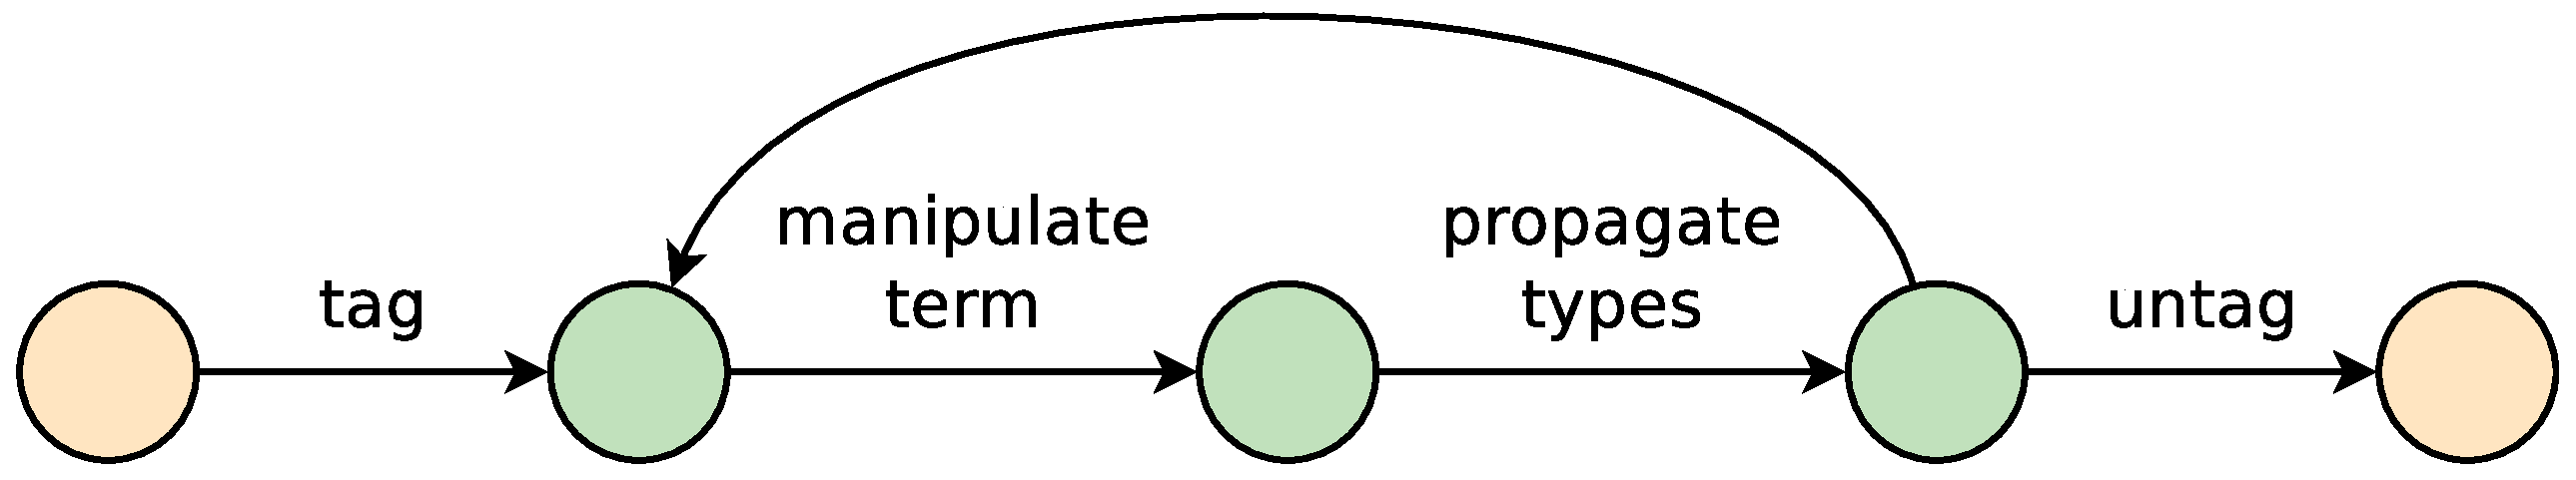
\includegraphics[width=0.8\textwidth]{propagation.eps}
    \caption{Illustration of a term manipulation process. Orange nodes
        represent typed $\lambda$-terms, while green nodes represent
        type-tagged $\lambda$-terms.}
    \label{fig:propagation}
}\fixednote{Тази фигура няма ли да се опрости, ако махнеш $\varepsilon$-преходите?}

We will informally assume that term manipulations don't alter semantics\footnote{
    by much} (in a very broad sense).

This ``type-tagged term'' construction \fixednote{моля поясни: tagging? manipulation? propagation?} does not need to include casts, since we are storing
a type for every subterm anyway, which can replace the use of casts for all
practical\footnote{
    There is no way to preserve multiple consecutive casts.
} cases. There is also no need for storing the types of bound variables, since
they can be easily extracted from the types of the respective abstraction terms.
\begin{defn}
    Let $C \subset \const$ be a set of constants, typed in $T$.

    The set of type-tagged $\lambda$-terms $\ttlambda{T}{C}$ is defined inductively\footnote{
        Here we use $\ttt{ M}{ \tau }$ instead of $M^\tau$
        to denote type tags in order not to confuse them with Church-style
        typing, which would imply that types are always correct (which we
        don't require here).
    }\fixednote{стандартната нотация за типове по термовете май е $M^\tau$. Ако нарочно въвеждаш различна нотация, за да разграничиш type-tagging от експлицитни системи стил Church, добре е да го кажеш явно.}:
    \begin{itemize}
        \item Constant:
            \[ c \in C, \tau \in \tclos{T} \implies \ttt{c}{\tau} \in \ttlambda{T}{C} \]
        \item Variable:
            \[ v \in \lvars, \tau \in \tclos{T} \implies \ttt{v}{\tau} \in \ttlambda{T}{C} \]
        \item Application:
            \[ A, B \in \ttlambda{T}{C}, \tau \in \tclos{T} \implies \ttt{(AB)}{\tau} \in \ttlambda{T}{C} \]
        \item Abstraction:
            \[ v \in \lvars, A \in \ttlambda{T}{C},
                \tau = (\tau' \tot \tau'') \in \tclos{T},
                \implies \ttt{(\lambda v \abstr A)}{\tau} \in \ttlambda{T}{C} \]
    \end{itemize}
\end{defn}

This construction is completely equivalent to the regular typed $\lambda$-term
construction (type-tags may be emulated by inserting casts at all subterms),
and is used only for convenience: this way we can manipulate types directly
instead of having to deal with casts and bound variable types.

Converting regular $\lambda$-terms into type-tagged $\lambda$-terms is
relatively straightforward: simply examine the type of every subterm according
to its local context and then store it into the tag.

Note that all functions that follow are partial since they are not defined for
valid but inadequately typed terms. In implementations,
encountering an ``undefined'' case in any of them is treated as a type error.

\greenbox{
    We will use the notation ``$\pfun$'' for denoting partial functions.
}

\begin{defn}
    \label{def:ttag}
    For a context $\Gamma$,
    $\mcf{tag}_{\Gamma} : \fancylambda{T}{C} \pfun \ttlambda{T}{C}$
    is defined inductively:
    \[
        \mcf{tag}_{\Gamma}(A) =
        \begin{cases*}
            \ttt{c}{\typeof{C}} ,& $A = c \in C$, \\
            \ttt{v}{\tau} ,& $A = v \in \lvars, \Gamma \vdash v : \tau$, \\
            \ttt{(\mcf{tag}_{\Gamma}(M) \app \mcf{tag}_{\Gamma}(N))}{\tau}
 ,& $A = (MN), \Gamma \vdash A : \tau$, \\
            \ttt{\lambda v \abstr \mcf{tag}_{\Gamma'}(M)}{\sigma \tot \tau}
 ,& $A = (\lambda v: \sigma \abstr M)
                 , \Gamma' \vdash M : \tau
                 , \Gamma' = \Gamma \circ v : \sigma$,\\
            \ttt{M}{\tau} ,& $A = \tau[M]$. \\
        \end{cases*}
    \]
\end{defn}

Although terms returned by $\mcf{tag}_{\Gamma}$ are well-typed (the unique type of
each subterm according to $\Gamma$ matches its tag), we want to manipulate
those terms before untagging them, and such manipulations may induce discrepancies
between actual types and type tags. Thus, our $\mcf{untag}_{\Gamma}$ function
will take extra care and insert casts where needed:
\begin{defn}
    For a context $\Gamma$,
    $\mcf{untag}_{\Gamma} : \ttlambda{T}{C} \pfun \fancylambda{T}{C}$
    and
    $\mcf{untag'}_{\Gamma} : \ttlambda{T}{C} \pfun \fancylambda{T}{C}$
    are defined inductively:
    \[
        \mcf{untag'}_{\Gamma}(\ttt{A}{\tau}) =
        \begin{cases*}
            c ,& $A = c \in C$, \\
            v ,& $A = v \in \lvars$, \\
            \mcf{untag}_{\Gamma}(P) \app \mcf{untag}_{\Gamma}(Q)
 ,& $A = (PQ)$, \\
            \lambda v : \tau' \abstr \mcf{untag}_{\Gamma'}(P)
 ,& $A = (\lambda v \abstr P), \tau = (\tau' \tot \tau'')
                 , \Gamma' = \Gamma \circ v : \tau'$. \\
        \end{cases*}
    \]

    \[
        \mcf{untag}_{\Gamma}(\ttt{A}{\tau}) =
        \begin{cases*}
            M ,& $M = \mcf{untag'}_{\Gamma}(\ttt{A}{\tau}), \Gamma \vdash M : \tau$, \\
            \tau[M] ,& $M = \mcf{untag'}_{\Gamma}(\ttt{A}{\tau}), \Gamma \not\vdash M : \tau$. \\
        \end{cases*}
    \]
\end{defn}

It can be easily seen that terms returned by $\mcf{untag}$ are well-typed,
since we've inserted casts wherever the types don't match. Note that $\mcf{untag}$
may be undefined in some cases (when its definition produces an invalid cast).
This means that it was given a term whose type cannot be cast to its type-tag.
We will assume that manipulations done to the term will not produce such cases.

Now that we have the construction for attaching types to subterms, we can
describe a universal way to propagate information through those types.\fixednote{няма ли да покажеш, че термовете, които се връщат от $\mcf{untag}$ са коректно типизирани?}

We will use a basic operation $\unify$ that unifies two types.

\begin{defn}
    An operation $ \unify : \tclos{T} \times \tclos{T} \pfun \tclos{T}$ is
    called a \emph{unifier} for $T$ if:\fixednote{защо не опишеш свойствата формално? мотивиращ пример за унификатор?}
    \begin{itemize}
        \item it is only defined for types with identical syntactic structure and
            preserves it, i.e. $\sigma \unify \tau = \nu$ implies that $\sigma$,
            $\tau$ and $\nu$ have the same syntactic structure\footnote{
                See \cref{def:typesynstruct}
            }.

        \item it is symmetric\footnote{
                Everything in this section may also be done for asymmetric unifiers.
                Since the need for them has not yet arisen, symmetricity has been
                assumed for simplicity.
            }:
            \[ \sigma \unify \tau = \nu \implies \tau \unify \sigma = \nu \]

        \item it is idempotent:
            \[ \forall \sigma \in \tclos{T} (\sigma \unify \sigma = \sigma) \]
    \end{itemize}
\end{defn}

A great example for a unifier is the type inference unifier defined in
\cref{sec:typeinf}.


It can also be extended for contexts in the following way:
\[
    \begin{split}
        \Gamma' \unify \Gamma'' \defeq
        &\{ (x : \sigma \unify \tau) \mid (x : \sigma) \in \Gamma', (x : \tau) \in \Gamma''\} \\
        \cup &
        \{ (x : \sigma) \mid (x : \sigma) \in (\Gamma' \cup \Gamma''),
            (x : \cdot) \not\in \Gamma',
            (x : \cdot) \not\in \Gamma'' \}. \\
    \end{split}
\]

Now, type propagation will be done in two steps: upward (propagating
information up the term tree and into the context) and downward (propagating
information down the term tree towards the leaves).

\begin{defn}
    \label{def:propagation}
    For a set of type symbols $T$ and a unifier for $T$ $\unify$, the functions
    $\mcf{up}_{\unify}$ that maps a type-tagged term into a new type-tagged term and
    an inferred context for its free variables, and $\mcf{down}_{\unify}$ that maps
    a type-tagged term, a desired type and a free variable context into a
    new type-tagged term, are defined inductively as follows:
    \[
        \mcf{up}_{\unify}(\ttt{A}{\tau}) =
        \begin{cases*}
            (\ttt{c}{\tau}, \{ \}) ,& $A = c \in C$ \\
            (\ttt{v}{\tau}, \{ v : \tau \}) ,& $A = v \in \lvars$ \\
            (\ttt{\lambda x \abstr \ttt{M}{\sigma'}}{(\eta' \unify \eta) \tot (\sigma' \unify \sigma)}, \Gamma')
 ,& $A = (\lambda x \abstr P)
                , \tau = (\eta \tot \sigma),$ \\
                \phantom{} &\phantom{, }$(\ttt{M}{\sigma'}, \Gamma) = \mcf{up}_{\unify}(P)
                , \Gamma' = \Gamma \setminus (x : \eta'),$ \\
                \phantom{} &\phantom{, }$(x : \eta') \in \Gamma$ \\
            (\ttt{\lambda x \abstr \ttt{M}{\sigma'}}{\eta \tot (\sigma' \unify \sigma)}, \Gamma')
 ,& $A = (\lambda x \abstr P)
                , \tau = (\eta \tot \sigma),$ \\
                \phantom{} &\phantom{, }$(\ttt{M}{\sigma'}, \Gamma) = \mcf{up}_{\unify}(P)$ \\
                \phantom{} &\phantom{, }$(x : \cdot) \not\in \Gamma$ \\
            (\ttt{P' Q'}{\sigma'' \unify \tau}, \Gamma_P \unify \Gamma_Q)
 ,& $A = (PQ), (P', \Gamma_P) = \mcf{up}_{\unify}(P),$ \\
                \phantom{} &\phantom{, }$(Q', \Gamma_Q) = \mcf{up}_{\unify}(Q), P' = \ttt{M}{\sigma' \tot \sigma''}$ \\
        \end{cases*}
    \]
    \[
        \mcf{down}_{\unify}(\ttt{A}{\tau}, \tau', \Gamma) =
        \begin{cases*}
            \ttt{c}{\tau \unify \tau'} ,& $A = c \in C$ \\
            \ttt{v}{\tau \unify \tau' \unify \tau''}
 ,& $A = v \in \lvars, (v : \tau'') \in \Gamma$ \\
            \ttt{\lambda x \abstr P'}{\tau''}
 ,& $A = (\lambda x \abstr P), \tau'' = \tau \unify \tau'$ \\
                \phantom{} &\phantom{, } $\tau'' = (\sigma \tot \eta), P' = \mcf{down}_{\unify}(P, \eta, \Gamma \circ (x : \sigma)),$ \\
            \ttt{P' Q'}{\tau''}
 ,& $A = (PQ), P = \ttt{M}{\sigma \tot \eta}, Q = \ttt{N}{\sigma'},$ \\
                \phantom{} &\phantom{, }$\tau'' = (\tau' \unify \tau), \sigma'' = (\sigma' \unify \sigma)$ \\
                \phantom{} &\phantom{, }$P' = \mcf{down}_{\unify}(P, (\sigma' \tot \tau''), \Gamma),
                Q' = \mcf{down}_{\unify}(Q, \sigma'', \Gamma)$ \\
        \end{cases*}
    \]

    For convenience, the function $\mcf{propagate}_{\unify}$ is defined as the combination
    of $\mcf{up}_{\unify}$ and $\mcf{down}_{\unify}$:
    \[
        \mcf{propagate}_{\unify}(P) = \mcf{down}_{\unify}(\ttt{M}{\tau}, \tau, \Gamma)
        \text{ , where } \mcf{up}_{\unify}(P) = (\ttt{M}{\tau}, \Gamma).
    \]
  \end{defn}
  \newpage
  \note{липсва стъпката за манипулиране на терм, може би е добре да дадеш поне един пример за такава функция? тук може би е редно да навържеш всички дефинирани функции в една обща функция, която работидиректно над $\lambda$-термове.}
\end{document}
